\documentclass{article}
\usepackage[utf8]{inputenc}

\usepackage{amsfonts}
\usepackage{amssymb}
\usepackage{amsmath}
\usepackage{amsthm}
\usepackage{enumitem}

\usepackage{bbold}
\usepackage{bm}
\usepackage{graphicx}
\usepackage{color}
\usepackage{hyperref}
\usepackage[margin=2.5cm]{geometry}

\begin{document}

% ==============================================================================

\title{\Large{INFO8006: Project 2 - Report}}
\vspace{1cm}
\author{\small{\bf Mr Pacman - s111111} \\ \small{\bf Miss Pacman - s222222}}

\maketitle

% ==============================================================================

\section{Bayes filter}

\begin{enumerate}[label=\alph*.,leftmargin=*]
    \item The sensor model describes the probability of observing a certain piece of evidence $E_t$ (a noisy distance measurement) given the true state $X_t$ (the ghost's position). The noise is modeled using a Binomial distribution. Let $X_t = (w, h)$ be the ghost's position and $X_p$ be Pac-Man's position. The true Manhattan distance is $d(X_t, X_p)$. The evidence $E_t$ is the true distance plus some noise: $E_t = d(X_t, X_p) + \text{noise}$. The noise itself is generated from a Binomial random variable $K \sim \text{Binomial}(n, p)$, where the noise is defined as $\text{noise} = K - np$. Substituting this into the evidence equation, we can solve for $K$:
    $$ K = E_t - d(X_t, X_p) + np $$
    The probability of observing evidence $E_t$ given the state $X_t$ is therefore the probability mass function (PMF) of the Binomial distribution for this value of $K$:
    $$ P(E_t | X_t) = \text{binom.pmf}(k=E_t - d(X_t, X_p) + np, n, p) $$
    where $n = \frac{\sigma^2}{p(1-p)}$ is derived from the sensor variance $\sigma^2$, and $p=0.5$.
    \item The unified transition model $P(X_{t+1} | X_t)$ describes the ghost's movement based on its fear of Pac-Man. This model is parameterized by a single "fear factor", let's call it $k_f$. Let $S(X_t)$ be the set of legal successor positions from the current position $X_t$. For any successor position $X_{t+1} \in S(X_t)$, a weight $w(X_{t+1})$ is assigned based on its distance to Pac-Man's position $X_p$:
    $$
    w(X_{t+1}) =
    \begin{cases}
        k_f & \text{if } d(X_{t+1}, X_p) \ge d(X_t, X_p) \\
        1 & \text{otherwise}
    \end{cases}
    $$
    where $d(\cdot, \cdot)$ is the Manhattan distance. The ghost prefers to move to positions that increase or maintain its distance from Pac-Man, and this preference is scaled by the fear factor $k_f$. The probability of transitioning to a specific successor $X_{t+1}$ is the normalized weight:
    $$ P(X_{t+1} | X_t) = \frac{w(X_{t+1})}{\sum_{X'_{t+1} \in S(X_t)} w(X'_{t+1})} $$
    This single model can represent all three ghost types by varying the parameter $k_f$:
    \begin{itemize}
        \item \texttt{confused}: $k_f = 1$ (moves almost randomly, as all legal moves have equal weight).
        \item \texttt{afraid}: $k_f = 2$ (has a slight preference to move away from Pac-Man).
        \item \texttt{scared}: $k_f = 8$ (has a strong preference to move away from Pac-Man).
    \end{itemize}
\end{enumerate}

\section{Implementation}

\begin{enumerate}[label=\alph*.,leftmargin=*]
    \item \textbf{\textit{Leave empty.}}
\end{enumerate}

\section{Experiment}

\begin{enumerate}[label=\alph*.,leftmargin=*]
    \item To summarize the uncertainty of Pacman's belief state $B$, we use its Shannon Entropy, defined as:
    $$ H(B) = - \sum_{x} P(x) \log_2 P(x) $$
    where the sum is over all positions $x$ in the maze. A high entropy value indicates that the probability is spread out over many positions, corresponding to high uncertainty. Conversely, a low entropy value indicates that the probability is concentrated in a small area, corresponding to high certainty.
    \item To measure the quality of the belief state, we use two metrics, assuming access to the ground truth ghost position $X_{true}$:
    \begin{itemize}
        \item \textbf{Position Error}: The Manhattan distance between the most likely position in the belief state (the one with the highest probability, $X_{belief}$) and the true ghost position.
        $$ \text{Error} = d(X_{belief}, X_{true}) $$
        A lower value indicates a more accurate belief.
        \item \textbf{Probability at Ground Truth}: The probability value that the belief state assigns to the true ghost position, $B(X_{true})$. A higher value indicates a better quality belief, as the filter correctly identifies the true location as being probable.
    \end{itemize}
    \item The experiments were conducted over 10 trials for each configuration, running for 100 timesteps. The following graphs show the mean of the metrics, with the shaded area representing one standard deviation.
    \begin{figure}[h!]
        \centering
        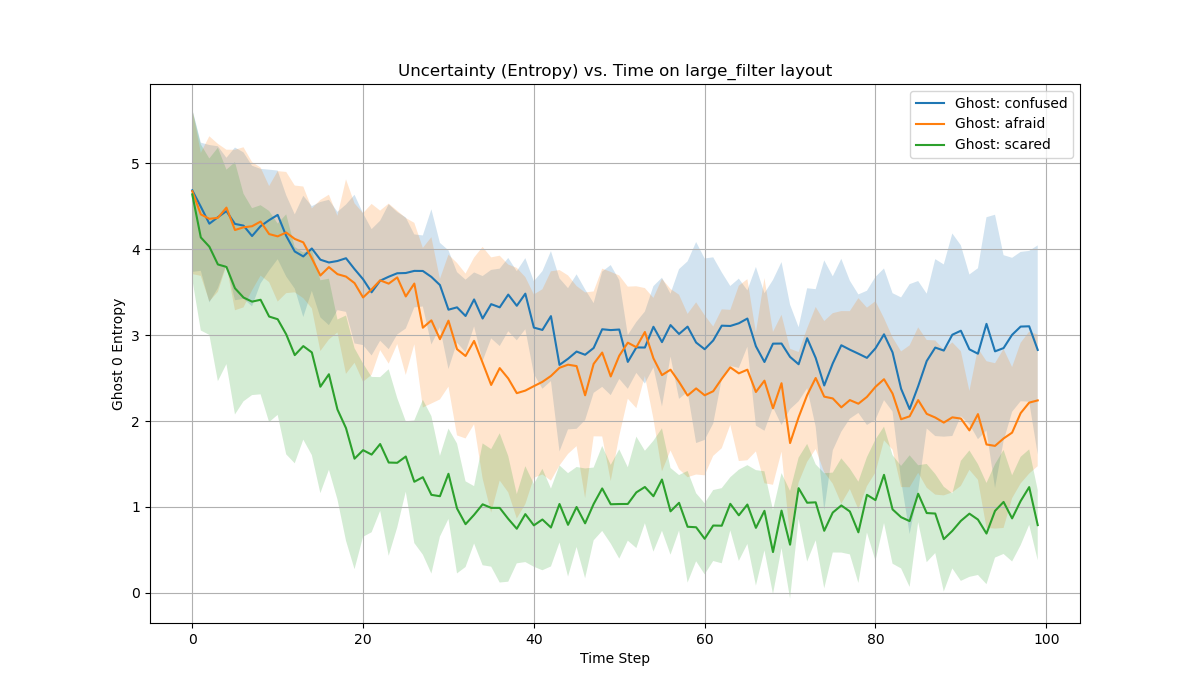
\includegraphics[width=0.8\textwidth]{graphs/entropy_large_filter.png}
        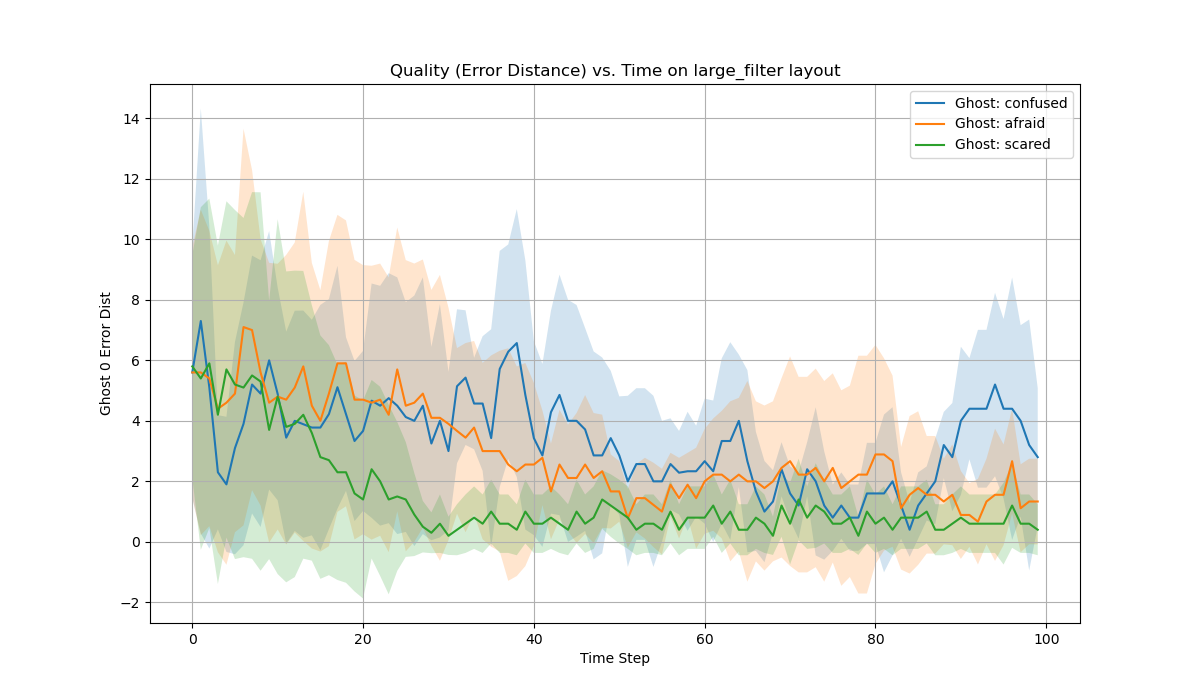
\includegraphics[width=0.8\textwidth]{graphs/error_dist_large_filter.png}
        \caption{Uncertainty (top) and Quality (bottom) on the \texttt{large\_filter} layout.}
    \end{figure}
    \begin{figure}[h!]
        \centering
        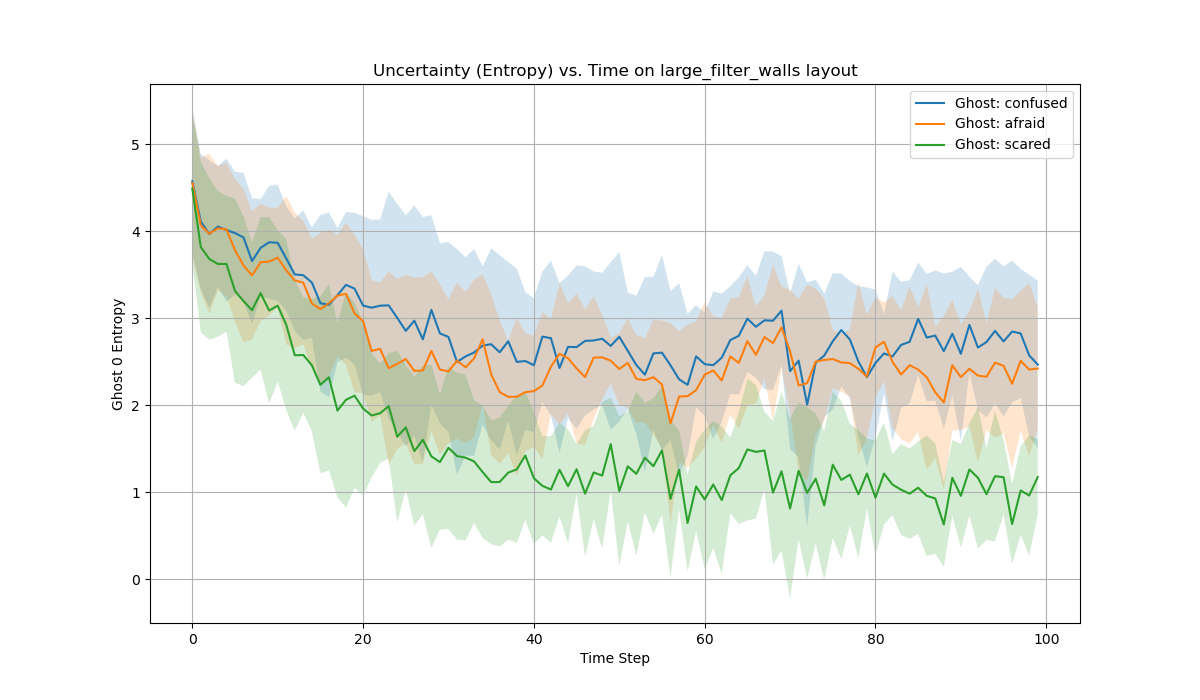
\includegraphics[width=0.8\textwidth]{graphs/entropy_large_filter_walls.png}
        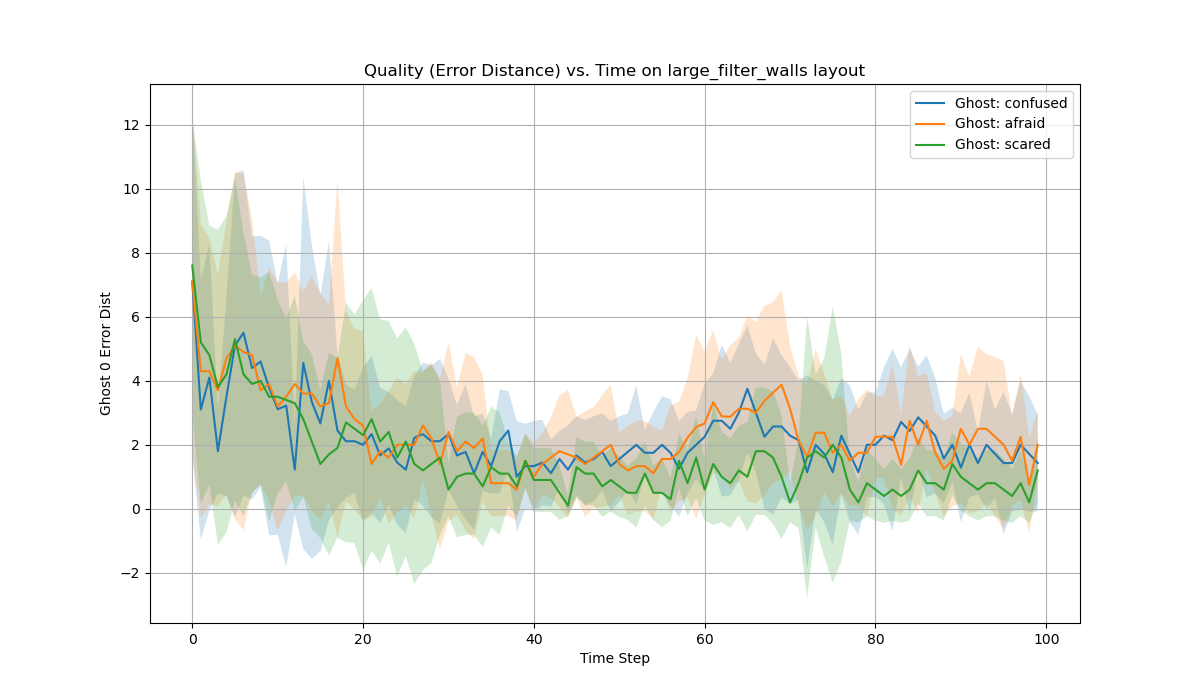
\includegraphics[width=0.8\textwidth]{graphs/error_dist_large_filter_walls.png}
        \caption{Uncertainty (top) and Quality (bottom) on the \texttt{large\_filter\_walls} layout.}
    \end{figure}
    
    \item \paragraph{3.d. Discuss the effect of the ghost transition model parameter on its own behavior and on Pacman's belief state.}
    The ghost's transition model parameter directly governs its level of "randomness" or unpredictability. This has a significant impact on both the ghost's behavior and Pacman's ability to track it, as evidenced by our entropy and error distance metrics across both layouts.
    
    Based on the model, a ghost like \texttt{scared} has a highly predictable transition model; it strongly prefers to move away from Pacman. This deterministic behavior results in a much narrower probability distribution for its next possible location. Conversely, the \texttt{confused} ghost has a more uniform transition model, making its movements far more random and harder to predict. The \texttt{afraid} ghost lies somewhere in between.
    
    Our graphical results strongly support this analysis. In both the \texttt{large\_filter} and \texttt{large\_filter\_walls} layouts, the \texttt{scared} ghost (blue line) consistently yields the lowest entropy and error distance. This indicates that Pacman maintains a highly confident and accurate belief state. The filter can effectively predict the ghost's next move, causing the belief state to converge quickly.
    
    For the \texttt{confused} ghost (green line), the entropy and error distance are consistently the highest. The randomness in its movement means that at each time step, the probability of the ghost's next position is spread across a wider area. This makes it challenging for the Bayes filter to reduce uncertainty, resulting in a less confident and less accurate belief state throughout the experiment.
    
    Comparing the layouts, we observe that both entropy and error distance are generally lower in the \texttt{large\_filter\_walls} layout. The presence of more walls restricts the possible movements for all ghost types, effectively reducing the branching factor of possible next states. This constraint aids the filter by pruning the hypothesis space, leading to a faster convergence and a more accurate belief state for all ghost types compared to the more open \texttt{large\_filter} layout.

    \item \paragraph{3.e. Discuss the effect of the sensor variance on Pacman's belief state.}
    The sensor variance is a critical parameter in the sensor model that defines the reliability of Pacman's measurements. It quantifies the "noise" or uncertainty in the sensor readings. A low variance implies a reliable sensor, while a high variance indicates a noisy, less trustworthy sensor.
    
    A \textbf{low sensor variance} would cause the likelihood distribution (from the sensor model) to be sharply peaked around the measured distance. When this evidence is incorporated into the Bayes filter, it has a strong corrective effect on the belief state. The filter will heavily weigh the sensor reading, causing the updated belief to converge very quickly to a small, confident area. The resulting entropy would decrease rapidly, and the error distance would be low, assuming the sensor is accurate.
    
    Conversely, a \textbf{high sensor variance} would result in a flatter, more spread-out likelihood distribution. This indicates that a wide range of ghost positions could plausibly explain the sensor reading. When this uncertain evidence is multiplied with the prior belief, it has a weaker corrective effect. The belief update step would be less effective at reducing uncertainty, causing the entropy to decrease much more slowly. Consequently, Pacman's belief state would remain more diffuse for a longer period, and the error distance would likely be higher, as the filter cannot confidently pinpoint the ghost's location.
    
    In essence, increasing the sensor variance would degrade the filter's performance, making Pacman less certain (higher entropy) and less accurate (higher error distance) about the ghosts' positions over time.

    \item \paragraph{3.f. How would you implement a Pacman controller to eat ghosts?}
    To implement a Pacman controller that actively hunts ghosts, one could design a policy that selects actions to minimize the distance to the most likely ghost position while also trying to improve its own belief state. A possible approach would be an expectimax-style agent.
    
    The agent would evaluate each legal action from its current state. For each action, it would project the consequences by considering:
    \begin{enumerate}
        \item \textbf{The most likely ghost location:} The primary goal is to eat the ghost. The agent could identify the cell $(x, y)$ with the highest probability in its current belief state, $B(X_t)$, and choose an action that minimizes the Manhattan distance to that cell.
        \item \textbf{Future uncertainty:} A more sophisticated agent would also consider how an action might improve future belief states. After moving to a new position, Pacman will receive a new sensor reading. The agent could choose actions that lead to positions where the expected future entropy is lowest. For example, moving to a location that is geometrically central to the high-probability region of the belief state might provide a more informative sensor reading in the next step.
        \item \textbf{Value of eating the ghost:} The state evaluation function would assign a very high reward to states where Pacman's position coincides with the most likely ghost position (i.e., when a ghost is eaten) and a small negative reward for each time step to encourage efficiency.
    \end{enumerate}
    The controller would then select the action that leads to the highest expected utility, balancing the short-term goal of getting closer to the ghost with the long-term goal of maintaining a confident belief state.
    
    \item \textbf{\textit{Leave empty.}}
\end{enumerate}

% ==============================================================================

\end{document}